\section{\Large Desarrollo}

\begin{enumerate}
	\subsection{Obteniendo los datos.}
	\item Ubicar la Estación Base (Base Station - BS), cuya ubicación es 19.503668573568277, -99.1279845883227. Usando Google Maps o por inspección directa estimar la altura a la que se encuentran colocadas las antenas.
	      \begin{figure}[H]
		      \centering
		      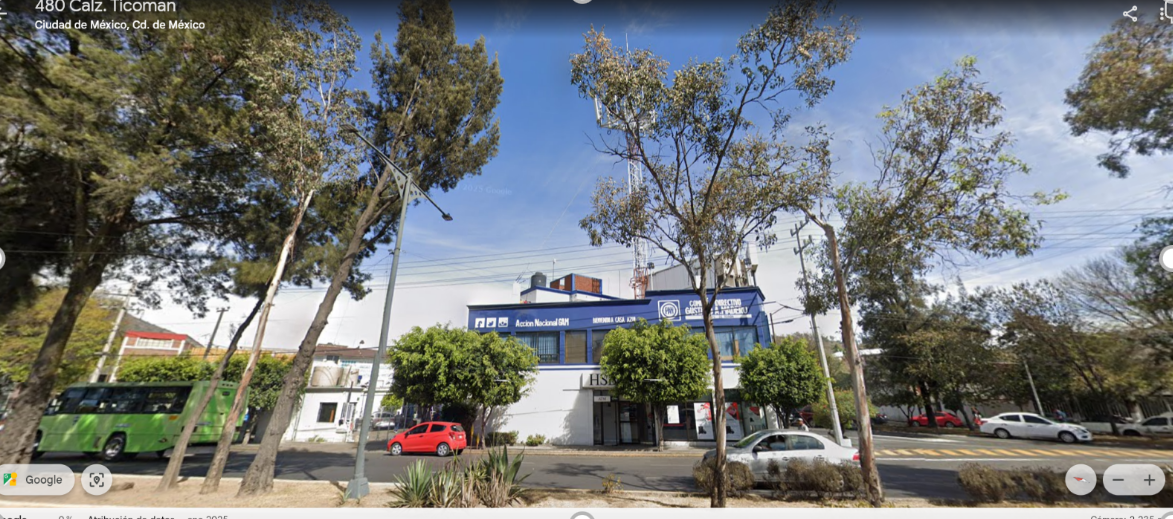
\includegraphics[width=0.9\textwidth]{./img/bs.png}
		      \caption{Imagen de la estación base en las coordenadas dadas.}
		      \label{fig:bs}
	      \end{figure}
	\item Trazar una línea recta entre la BS y la coordenada asignada y calcular la potencia recibida por cada intersección entre una calle y la línea trazada considerando los modelos espacio libre, superficie reflejante, COST231 Walfish-Ikegami y lognormal.
	      \textbf{Coordenadas: 19.508953097456004, -99.12414451054960}
	      \begin{figure}[H]
		      \centering
		      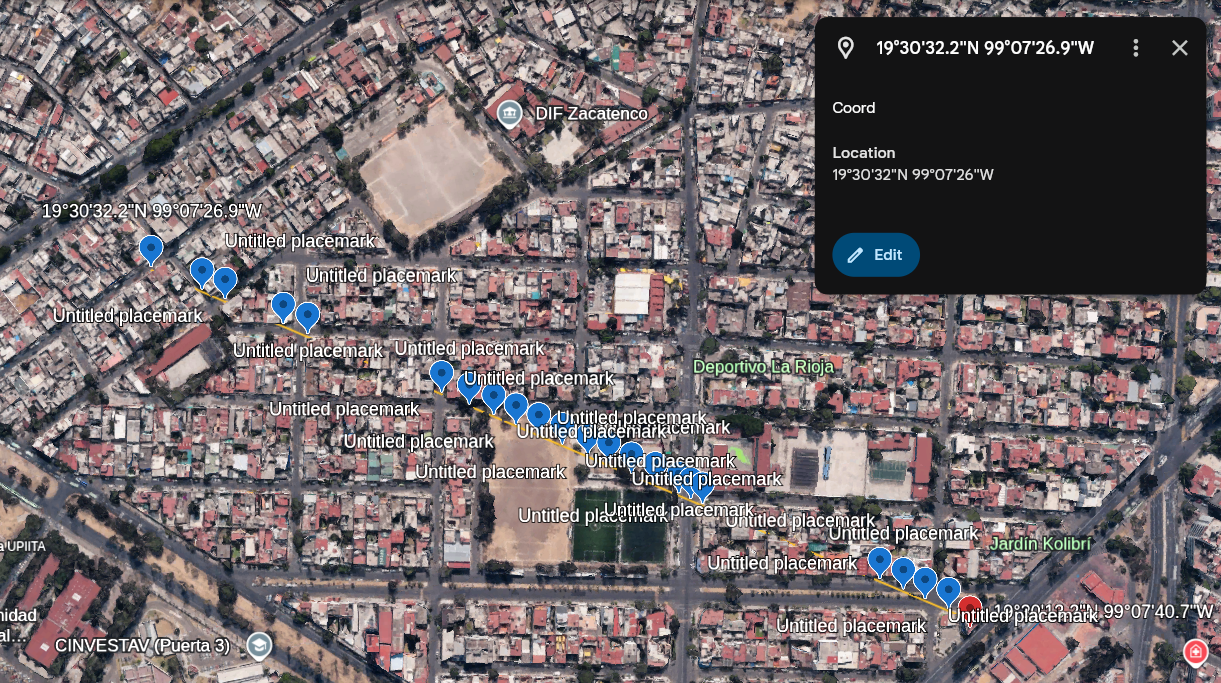
\includegraphics[width=0.9\textwidth]{./img/coordenada-dada.png} % Ajusta el ancho
		      \caption{Línea recta desde la BS hasta la coordenada asignada.}
		      \label{fig:coordenada-dada}
	      \end{figure}

	      \begin{figure}[H]
		      \centering
		      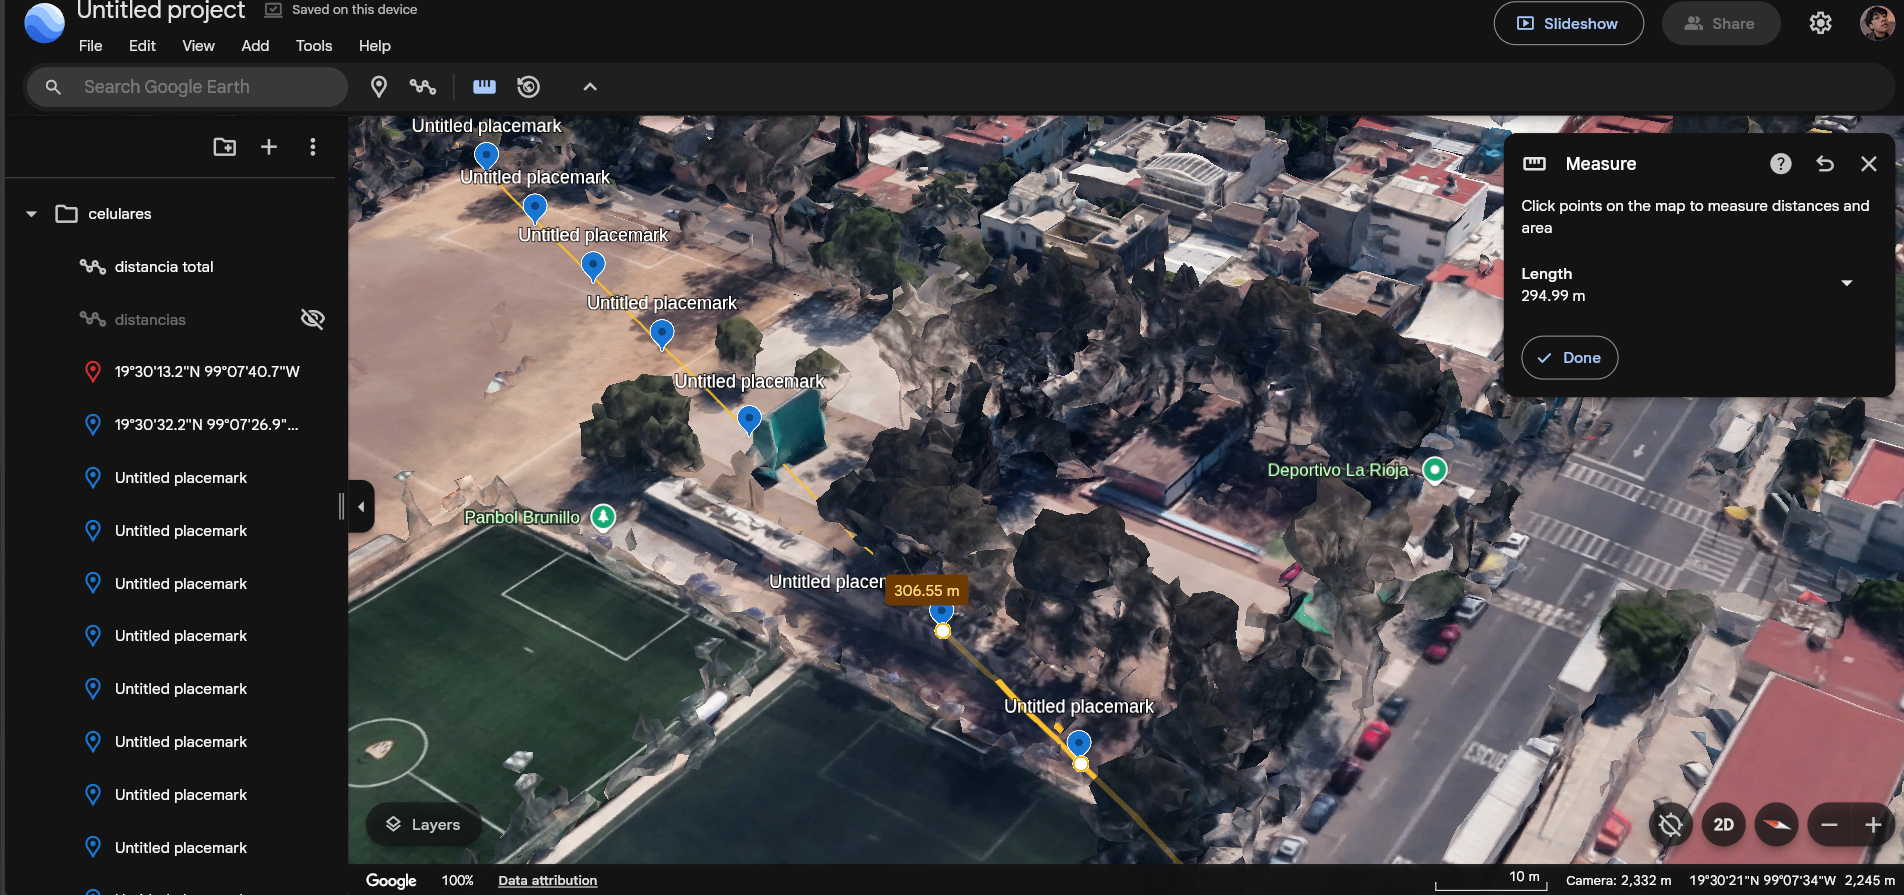
\includegraphics[width=0.9\textwidth]{./img/distancias-puntos.png} % Ajusta el ancho
		      \caption{Sacando las distancias de la BS a cada punto (aprox cada 20m en exteriores).}
		      \label{fig:distancias-puntos}
	      \end{figure}
	      \begin{figure}[H]
		      \centering
		      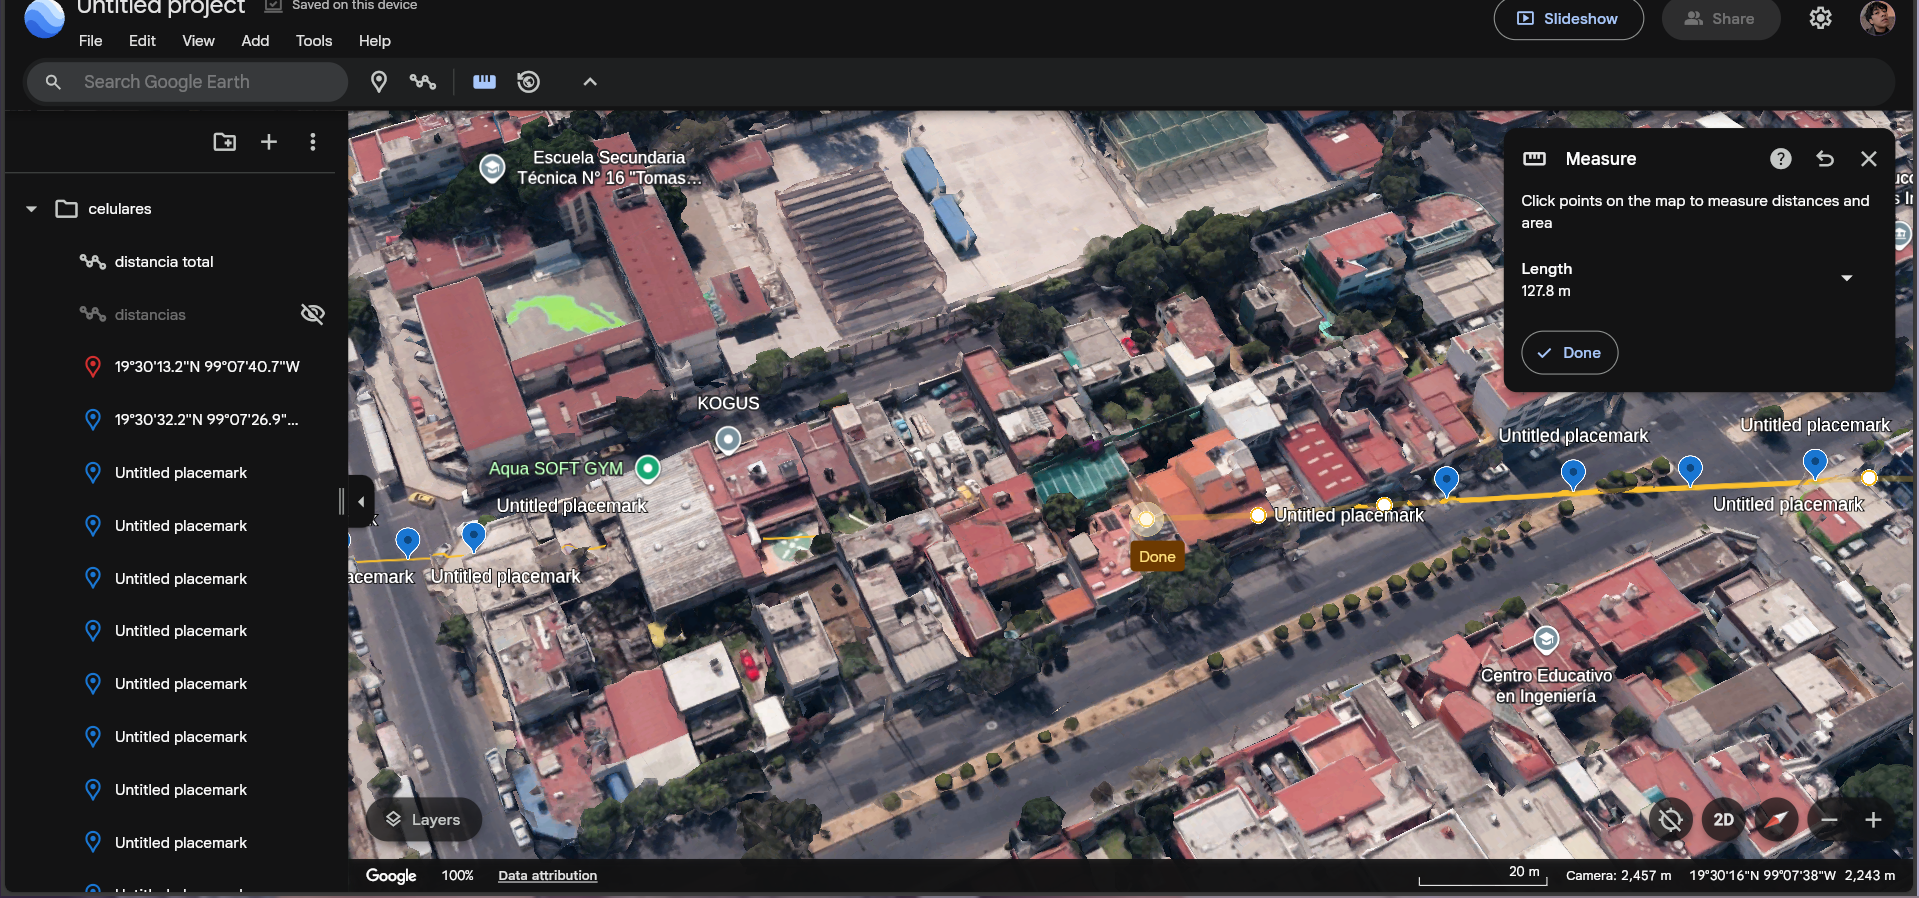
\includegraphics[width=0.9\textwidth]{./img/distancias-edificios.png} % Ajusta el ancho
		      \caption{Sacando las distancias de los edificios.}
		      \label{fig:distancias-edificios}
	      \end{figure}
	\item Considerar una frecuencia de operación de 1,935 MHz para los modelos que lo requieran. Además, considerar que la potencia de transmisión es de 10W y que las ganancias de las antenas transmisora y receptora son 9 y 3 dB, respectivamente.
	\item Para el modelo COST231 Walfish-Ikegami realizar una tabla con los siguientes datos por cada punto analizado:
	      \begin{enumerate}
		      \item Coordenadas
		      \item Distancia a la EB
		      \item Si existe LOS o no
		      \item Separación promedio entre edificios, b (si aplica).
		      \item Ancho de la “calle” en la que se encuentra el móvil, w (si aplica).
		      \item Altura promedio de edificios, h (si aplica)
		      \item Ángulo de orientación, $\phi$ (si aplica).
		      \item $L_0.$
		      \item $L_{rts}$. (Si aplica).
		      \item $L_{msd}$. (Si aplica).
		      \item Potencia recibida (en dBm)
	      \end{enumerate}
	      \begin{table}[H]
		      \centering
		      \resizebox{\textwidth}{!}{%
			      \begin{tabular}{|c|c|c|c|c|c|c|c|c|c|c|}
				      \hline
				      \textbf{Coordenadas} & \textbf{Distancia a la EB} & \textbf{LOS} & \textbf{b (m)} & \textbf{w (m)} & \textbf{h (m)} & \textbf{$\Phi$ (°)} & \textbf{L$_0$ (dB)} & \textbf{L$_{rts}$ (dB)} & \textbf{L$_{msd}$ (dB)} & \textbf{P$_{rec}$ (dBm)} \\
				      \hline
				                           &                            &              &                &                &                &                     &                     &                         &                         &                          \\
				      \hline
				                           &                            &              &                &                &                &                     &                     &                         &                         &                          \\
				      \hline
			      \end{tabular}%
		      }
		      \caption{Parámetros de propagación para diferentes ubicaciones}
		      \label{tab:parametros_propagacion}
	      \end{table}
	\item Para el modelo lognormal, considere $\alpha$=2.8 y $\sigma$=7dB y realizar una tabla con los siguientes datos por cada punto analizado:
	      \begin{enumerate}
		      \item Coordenadas
		      \item Distancia a la EB
		      \item Pérdidas por distancia
		      \item Pérdidas por ensombrecimiento
		      \item Potencia recibida (en dBm)
	      \end{enumerate}
	      \begin{table}[H]
		      \centering
		      \resizebox{\textwidth}{!}{%
			      \begin{tabular}{|c|c|c|c|c|}
				      \hline
				      \textbf{Coordenadas} & \textbf{Distancia a la EB (m)} & \textbf{Pérdidas por distancia (dB)} & \textbf{Pérdidas por ensombrecimiento (dB)} & \textbf{P$_{rec}$ (dBm)} \\
				      \hline
				                           &                                &                                      &                                             &                          \\
				      \hline
				                           &                                &                                      &                                             &                          \\
				      \hline
				                           &                                &                                      &                                             &                          \\
				      \hline
			      \end{tabular}
		      }
		      \caption{Parámetros del modelo lognormal con $\alpha=2.8$ y $\sigma=7$ dB}
		      \label{tab:modelo_lognormal}
	      \end{table}

	\item  Realizar una figura en la que muestre la potencia recibida en función de la distancia para cada uno de los modelos y escribir un análisis de estos resultados


\end{enumerate}